\documentclass[acmsmall,10pt,review,anonymous]{acmart}\settopmatter{printfolios=true,printccs=false,printacmref=false}
\usepackage{booktabs,listings,xspace,wrapfig}
\lstset{language=R}
\usepackage{my_style}
\definecolor{LightGray}{rgb}{.95,.95,.95}
\definecolor{Gray}{rgb}{.3,.3,.3}
\definecolor{DarkGray}{rgb}{.5,.5,.5}

\graphicspath{ {./plots/} }

\lstset{ %
  columns=flexible,
  captionpos=b,
  frame=single,
  framerule=0pt,
  framexleftmargin=-1mm,
  framexrightmargin=-1mm,
  tabsize=2,
  belowskip=0pt,
  basicstyle=\small\ttfamily,
  backgroundcolor=\color{LightGray},
  emphstyle=\sffamily,
  keywordstyle=\bfseries,
  commentstyle=\color{Gray}\em,
  stringstyle=\color{Gray},
 % numbers=left
}

\lstdefinestyle{R}{ %
  language=R,
  deletekeywords={env, equal, c, runif, trace, args},
  breaklines=true
}

\lstdefinestyle{Rin}{ %
  style=R,
  numberstyle=none,
  basicstyle=\normalsize\ttfamily,
  breaklines=false
}

\newcommand{\code}[1]{\lstinline|#1|\xspace}
\newcommand{\genthat}{{\sc Genthat}\xspace}

% Macros for type names?
\newcommand{\reals}{$\mathtt {\rm I\!R}$\xspace}
\newcommand{\realv}{$\overline{\rm I\!R}$\xspace}

\setcopyright{none}
%\setcopyright{acmcopyright}%\setcopyright{acmlicensed}
%\acmDOI{10.475/123_4}
%\acmConference[OOPSLAs]{Woodstock conference}{July 1997}{El Paso, Texas USA}
%\acmYear{1997}%\copyrightyear{2016}%\acmPrice{15.00}
\begin{document}

\title{A Large-Scale Study of Polymorphism in R}

\newcommand{\PACKAGES}{11,463\xspace}
\newcommand{\PROGRAMMERS}{?\xspace}
\newcommand{\PERCENTCRAN}{83\%\xspace}
\newcommand{\CRANTOTAL}{13,841\xspace}
\newcommand{\RLOC}{15,050,267\xspace}
\newcommand{\CLOC}{9,373,542\xspace}
\newcommand{\YEARS}{20\xspace}
\newcommand{\INDEXCOINCIDENCE}{3,499\xspace}
\newcommand{\TOTALINDEXY}{6,561\xspace}
\newcommand{\INDEXYPERC}{53\%\xspace}		% TODO Not an accurate count.
\newcommand{\DATAPKGS}{206\xspace}
\newcommand{\DATAPKGSPERC}{1.5\%\xspace}
\newcommand{\METAARGCOUNT}{7,051\xspace}
\newcommand{\NUMPOLYTYPEMONOCLASS}{1,357\xspace}
\newcommand{\PERCSCALARMONO}{37.6\%\xspace}

\newcommand{\LZEROPERCPOLY}{17\%\xspace}
\newcommand{\LONEPERCPOLY}{20.4\%\xspace}
\newcommand{\LTWOPERCPOLY}{23\%\xspace}

\newcommand{\attr}[2]{\ensuremath{#1_{\mathtt{#2}}}\xspace}
\newcommand{\attrclass}[3]{\ensuremath{#1^{\mathtt{#3}}_{\mathtt{#2}}}\xspace}
\renewcommand{\to}{\ensuremath{\rightarrow}\xspace}
\newcommand{\D}{\ensuremath{\small\vec{\mathtt D}}\xspace} % Double
\newcommand{\I}{\ensuremath{\small\vec{\mathtt I}}\xspace} % Integer
\renewcommand{\C}{\ensuremath{\small\vec{\mathtt C}}\xspace} % Character
\renewcommand{\L}{\ensuremath{\small\vec{\mathtt L}}\xspace} % Logical
\newcommand{\R}{\ensuremath{\small\vec{\mathtt R}}\xspace} % Raw
\newcommand{\X}{\ensuremath{\small\vec{\mathtt X}}\xspace} % Complex
\newcommand{\Y}{\ensuremath{\small\vec{\mathtt Y}}\xspace} % Symbol
\newcommand{\sY}{\ensuremath{\small{\mathtt Y}}\xspace} % Symbol
\newcommand{\sS}{\ensuremath{\small{\mathtt S}}\xspace} % S4
\newcommand{\sF}{\ensuremath{\small{\mathtt F}}\xspace} % Closure
\newcommand{\sE}{\ensuremath{\small{\mathtt E}}\xspace} % Env
\renewcommand{\R}{\ensuremath{\small\vec{\mathtt R}}\xspace} % Raw
\newcommand{\sN}{\ensuremath{\small{\mathtt N}}\xspace}     % Null
\renewcommand{\l}{\ensuremath{\small\underline{\mathtt ?}}\xspace}     % List
\newcommand{\sD}{\ensuremath{\small{\mathtt D}}\xspace} % Double
\newcommand{\sI}{\ensuremath{\small{\mathtt I}}\xspace} % Integer
\newcommand{\sC}{\ensuremath{\small{\mathtt C}}\xspace} % Character
\newcommand{\sL}{\ensuremath{\small{\mathtt L}}\xspace} % Logical
\newcommand{\sX}{\ensuremath{\small{\mathtt X}}\xspace} % Complex
\newcommand{\sR}{\ensuremath{\small{\mathtt R}}\xspace} % Raw
\newcommand{\ANY}{\ensuremath{\small{\mathtt ?}}\xspace}     % Any
\newcommand{\lT}[1]{\ensuremath{\small\underline{\mathtt #1}}\xspace}     % list<T>
\newcommand{\M}[1]{\ensuremath{\attr{\vec{\tt #1}}{mat}}\xspace}     % matrix
\newcommand{\df}{\ensuremath{\attr{\l}{df}}\xspace}     % data.frame




\begin{abstract}
The R programming language is widely used in a variety of scientific domains
for tasks related to data science. The language was designed to favor an
interactive style of programming with minimal syntactic and conceptual
overhead. This design is well suited to support interactive data analysis,
but is not well suited to generating performant code or catching programming
errors.  In particular, R has no type annotations and all operations are
dynamically checked at runtime. The starting point for our work is the
question: \emph{what could a static type system for R look like?}  To answer
that question we study the polymorphism that is present in \RLOC lines of R
code spread among some \PACKAGES packages, written over a
period of over \YEARS years by thousands of programmers.  We perform a dynamic
analysis, leveraging tests and use-cases, to determine the level of
polymorphism that is present in the code. We do this for several potential
notions of types. Our result suggest that polymorphism is important in some
key parts of the system but that relatively simple type annotations could be
used to capture most of the interesting cases.

\end{abstract}

\maketitle

\section{Introduction}

Our community builds, improves, and reasons about programming languages.  To
make design decisions that benefit most users, we need to understand the
language we are working with as well as the real-world needs it
answers. Often, we, as researchers, can appeal to our intuition as many
languages are intended to be general purpose and appeal to users with some
computer science training. Unfortunately, these intuitions don't always
apply to domain-specific languages, languages designed for and by a specific
group of users to solve very specific needs. This is the case of the data
science language R.

R and its ancestor S are languages designed, implemented and maintained by
statisticians. Originally they were designed as glue languages, languages
that would allow to read data into vectors and call statistical routines
written in Fortran. Over three decades, the languages became widely used
across many fields of science and in industry for data analysis and data
visualization; with time additional features were added.  Modern R, as a
linguistic object of study, is fascinating. It is a vectorized, dynamically
typed, lazy functional language with limited side-effects, extensive
reflective facilities and retrofitted object-oriented programming support.

Many of the design decisions that gave us R were intended to foster an
interactive, exploratory, programming style. This includes, to name a few,
the lack of type annotations on variables and functions, the ability to use
syntactic shortcut, and the automatic conversion between data types.  While
these choices have led to a language that is surprisingly easy to use by
beginners --many data science programs do not teach the language itself but
simply introduce some of its key libraries-- they have also created a
language where almost all computations yield a numeric result and where
errors can go undetected.

One way to increase assurance in the results obtained when using R would be
to add type annotations to functions and variable declarations. These
annotations could then be used, either statically or (more likely)
dynamically, to catch mismatches between expected and provided data values.
The nature of R is such that it is unlikely to be ever fully statically
checked, furthermore end users may not be willing to write types when
carrying out exploratory programming tasks. So, we are looking for an
optional type system that would allow us to capture as much of behavior of
library functions as possible while remaining easy to understand for
end-users and library developers alike.

This papers is a data-driven study of what a type system for the R language
could look like. Longer term, our intention is to propose changes to
language, but for any changes to be accepted by the user community, they
must clearly benefit the language without endangering backwards
compatibility. Our goal is thus to find a compromise between simplicity and
usefulness; the proposed type system should cover most common programming
idioms while remaining easy to use. In order to do this, we need to
understand the degree of polymorphism present in R code, that is to say, how
programmers leverage the dynamic nature of R to write code that can accept
arguments of different types.  This understanding will drive our design.

We propose to capture the degree of polymorphism present in R by the means
of a dynamic analysis of widely used libraries. For each function call we
can record the types of its arguments and of its return value. This allows
us to observe how many different combination of types are accepted by any
given function. Unlike many other languages, R has a carefully curated
software repository called CRAN. To be deposited in CRAN, a package must
come with sample dataset, tests and executable use-cases. As part of normal
operations these tests are run regularly and failing packages are removed.
This allowed us to have access to \PACKAGES libraries and about an order of
magnitude more runnable scripts that exercise those libraries.

The contributions of this paper are thus as follows:
\begin{itemize}
\item A large-scale analysis of the polymorphism present in function
  signatures of \PACKAGES widely used and actively maintained R packages.
\item A tracing and analysis pipeline that extends a previously published
  test generation tool named \genthat.
\item Manual analysis of 100 functions to validate the dynamic analysis
  results.
\end{itemize}

One threat to validity of our work is that we rely on dynamic analysis, so
our conclusions are only as good as the coverage of the possibly function
behaviors. Previous work~\cite{issta18}, reported that running all the
scripts that come with CRAN packages gives, on average, 68\% test coverage.
We attempted to mitigate the threat coming from the fact that only part of
the code is being exercised by manual analysis. It would be reasonable to
ask for confirmation of the data by static analysis of the code, but sound
static analysis of R is difficult because of the extensive use of reflective
features such as \code{eval} and of the ability to redefine the meaning of
operators such as \code{+} and \code{if}.  Another threat to validity is
that we only have access to code that has been deposited in the CRAN
repository. While this may bias our findings towards code written to be
reusable and, possibly, better engineered than typical user code. This is
also the code that would most benefit from type annotations.

\newpage  %%Leave here

\section{The R Programming Language}\label{sec:rlang}

Over the last decade, the R Project has become a key tool for implementing
sophisticated data analysis algorithms in fields ranging from Computational
Biology~\cite{R05} to Political Science~\cite{R:Keele:2008}. At the heart of
the R project is a \emph{vectorized, dynamic, lazy, functional,
  object-oriented} programming language with a rather unusual combination of
features~\cite{ecoop12} designed to ease learning by non-programmer and
enable rapid development of new statistical methods.  The language, commonly
referred to as R was designed in 1993 by Ross Ihaka and Robert
Gentleman~\cite{R96} as a successor to S~\cite{S88}.  First released in
1995, under a GNU license, R rapidly became the lingua franca for
statistical data analysis. Today, there are over 13,000 R packages available
from repositories such as CRAN and Bioconductor.  With 55 R user groups
world-wide, Smith~\cite{eco11} estimates that there are over 2 million
end-users.

As an introduction to R, consider the code snippet in Fig.~\ref{sample} from
a top-level interaction where the user defines a function \code{normSum}
that accepts vectors of integers, logicals, doubles and complex values and
normalizes the vector with respect to its sum and rounds the results. The
function definition does not require type annotations, and all operations
transparently work on vectors of any length and different types.

\begin{figure}[!hb]{\small
\begin{lstlisting}[style=R]
> normSum <- function( m )  round( m / sum(m), 2)
> normSum(c(1L,3L,6L))
[1] 0.1 0.3 0.6
> normSum(c(1.1,3.3,6.6))
[1] 0.1 0.3 0.6
> normSum(c(1.6,3.3,6.1))
[1] 0.15 0.30 0.55
> normSum(complex(r=rnorm(3),i=rnorm(3)))
[1] 0.49+0.21i 0.30-0.18i 0.22-0.03i
\end{lstlisting}}
\caption{Sample R code}\label{sample}
\end{figure}

In R, function can be called with named parameters, R support variable
argument lists, and arguments can have default values. Putting all of these
together consider the following declaration:

\begin{lstlisting}[style=R]
f <- function(x, ..., y=3) x + y
\end{lstlisting}

\noindent
Function \k{f} can be called with a single argument \code{f(3)}, with named
argument \code{f(y=4,x=2)} and with a variable number of arguments,
\code{f(1,2,3,4,y=5)}, all of these calls will return \code{6}.

R has a number of features that are not crucial to the present
discussion. We will mention some of them here for completeness.  In R, data
structures are reference counted and have copy-on-write semantics, thus the
assignment \code{x[12]<-3} results in an update to a copy of \code{x} unless
the reference count on that object is 1.  This semantics gives R a
functional flavor while allowing updating in place within loops (the first
update copies, subsequent updates are performed on the copy). Arguments to
functions are evaluated only when needed, they are bundled in so-called
promises which package the original expression (as an AST), its environment
as well as the result of evaluating the expression. Promises can be
leveraged for meta-programming as it is possible to retrieve the text of a
promise and evaluate that in a different environment.

\subsection{Types of Data}

Before attempting to define a type system for R, we should understand the
different kinds of values that programs operate on.  As we will see
different notions of type may emerge depending on how granular we want to
be.

\renewcommand{\k}[1]{{\tt #1}\xspace}

R has one builtin notion of type that can be queried by the \k{typeof}
function. Over the years, programmers have found the need for a richer type
structure and have added attributes. The best way to think of attributes is
as an optional map from name to values that can be attached to any object.
Attributes are used to encode various type structures. They can be queried
with functions such as \k{attributes} and \k{class}.

\begin{wrapfigure}{r}{6.1cm}
\footnotesize\begin{tabular}{l|c|l@{}}\hline
\multicolumn{3}{l}{\bf Vectorized data types:}  \\\hline
\k{logical}   & \L & vector of boolean values\\
\k{integer}   & \I & vector of 32 bit integer values\\
\k{double}    & \D & vector of 64 bit floating points\\
\k{complex}   & \X & vector of complex values\\
\k{character} & \C & vector of strings values\\
\k{raw}       & \R & vector of bytes\\
\k{list}      & \l & vector of values of any type\\\hline
\multicolumn{3}{l}{\bf Scalar data types:}\\\hline
\k{NULL}      & \sN &  singleton null value\\
\k{S4}        & \sS &  instance of a S4 class \\
\k{closure}   & \sF & a function with its environment\\
\k{environment}&\sE &  a mapping from symbol to value \\\hline
\multicolumn{3}{l}{\bf Implementation data types:}\\\hline
\multicolumn{3}{l}{\k{special},
\k{builtin},
\k{symbol} (\sY),
\k{pairlist},
\k{promise}}\\
\multicolumn{3}{l}{
\k{language},
\k{char},
\k{...},
\k{any},
\k{expression},
}\\
\multicolumn{3}{l}{
\k{externalprt},
\k{bytecode},
\k{weakref}}\\\hline
\end{tabular}\caption{Builtin Types}\label{types}\end{wrapfigure}

Figure~\ref{types} lists all of the builtin types that are provided by the
language. They are the possible return values of \k{typeof}. There is no
intrinsic notion of subtyping in R. But, in many context a \k{logical} will
convert to \k{integer}, and an \k{integer} will convert to \k{double}.  Some
off conversion can occur in corner cases, such as \k{1<"2"} holds and
\k{c(1,2)[1.6]} returns the first element of the vector, as the double is
converted to an integer. R does not distinguish between scalars and vectors
(they are all vectors), so \code{typeof(5) ==} \code{typeof(c(5)) ==
  typeof(c(5,5))} \code{ == "double"}. Finally all vectorized data types have a
distinguished missing value denoted by \code{NA}. The default type of
\code{NA} is \k{logical}. We can see that \code{typeof(NA)=="logical"}, but
NA inhabits every type: \code{typeof(c(1,NA)[2])=="double"}.

With one exception all vectorized data types are monomorphic, the exception
is the \k{list} type which can hold values of any other type including
\k{list}. For all monomorphic data types, attempting to store a value of a
different type will cause a conversion. Either the value is converted to the
type of vector, or the vector is converted to the type of the value.

Scalar data types include the distinguished \k{NULL} value, which is also of
type \k{NULL}, instance of classes written using the S4 object system,
closures and environments.  The implementation of R has a number of other
types that are mostly not used by user code, they are listed in
Figure~\ref{types} for reference.

The addition of attributes lets programmers extend the set of types by
tagging data with user-defined attributes. For example, one could define a
vector of four values, \code{x<-c(1,2,3,4)} and then attach the attribute
\k{dim} with a pair of numbers as value: \code{attr(x,"dim")<-c(2,2)}.  From
that point, arithmetic functions will treat \k{x} as a 2x2 matrix. Another
attribute that can be set is the \k{class}.  This attribute can be bound to
a list of class names. For instance, \code{class(x)<-"human"}, set the class
of \k{x} to be \k{human}.  Attributes are thus used for object-oriented
programming. The S3 object system support single dispatch on the class of
the first argument of a function, whereas the S4 object system allows
multiple dispatch (on all arguments). Some of the most widely used data
type, such as data frames, leverage attributes. A data frame, for instance,
is a list of vectors with a class and a column name attribute.

\paragraph{Summary.} The most common values in R computations are vectorized
types. R programs do not have a way to constrain values to be scalar.
\k{NULL} is sometimes used to represent the case when no value is
available. \k{NA} is used within vector to represent missing observations.
Attributes can decorate values and are used as building blocks for
object-oriented programming. A potential type system for R could focus only
on the builtin types, if one wanted to strive for simplicity, or it could
try to capture attributes at the risk of increased complexity.

\newpage
\section{Corpus}\label{sec:corpus}

In this section, we present our dataset. The R language aims to accommodate
data analysts; their workflows start with data import, followed by cleaning,
and then by steps of modeling, transformation and visualization. Often, the
code of these analysis pipelines resides, together with the data and
results, in notebooks. Few notebooks are publicly shared, and when they are,
the data isn't. For this reason our analysis focuses on packages which
bundle reusable units of R code with documentation, sample data and
use-cases.

We focus on packages hosted on the \emph{Comprehensive R Archive Network} or
CRAN.  With over 13,000 packages, CRAN is the largest repository of software
written in R. It is experiencing sustained growth with an average of size
new packages a day~\cite{LIgges2017}.  Unlike sites like GitHub, CRAN is a
\emph{curated} collection: A package is only accepted to CRAN if it abides
by a number of well-formedness rules.  Most relevant for our purposes,
packages must have data, examples, vignettes and tests, all of which must
successfully run. From our perspective this means that each package in CRAN
comes with several executable scripts that exercise some of its
functionality.  Notable exceptions to this rule are packages only containing
data, which have no runnable code but are referenced by other packages.
Only \DATAPKGS packages had no executable code, accounting for \DATAPKGSPERC
of CRAN.

The corpus used in this paper is a subset of CRAN. We retained packages that
could be run by our infrastructure in less than one hour. This corpus
consists of \PACKAGES packages, accounting for some \PERCENTCRAN of all
packages.  These packages have a total of \RLOC lines of R code and \CLOC
lines of C code. Figure~\ref{allcloc} shows a per-package breakdown of the
size of each package sorted by increasing numbers of lines of R. The figure
suggests that there is little correlation between the C/C++ parts and how
many lines of R a package contains. The median size of a package is 541
lines of R code and the largest package has 86K LOC. Typically, C/C++ code
is used to implement performance critical portions of the code. The majority
of package, 8,375 to be precise, have no C or C++ code.  The remaining 3,078
packages, have a median 572 lines of C and the largest package has 385,839
lines of C.

\begin{figure}[!b]\begin{center}
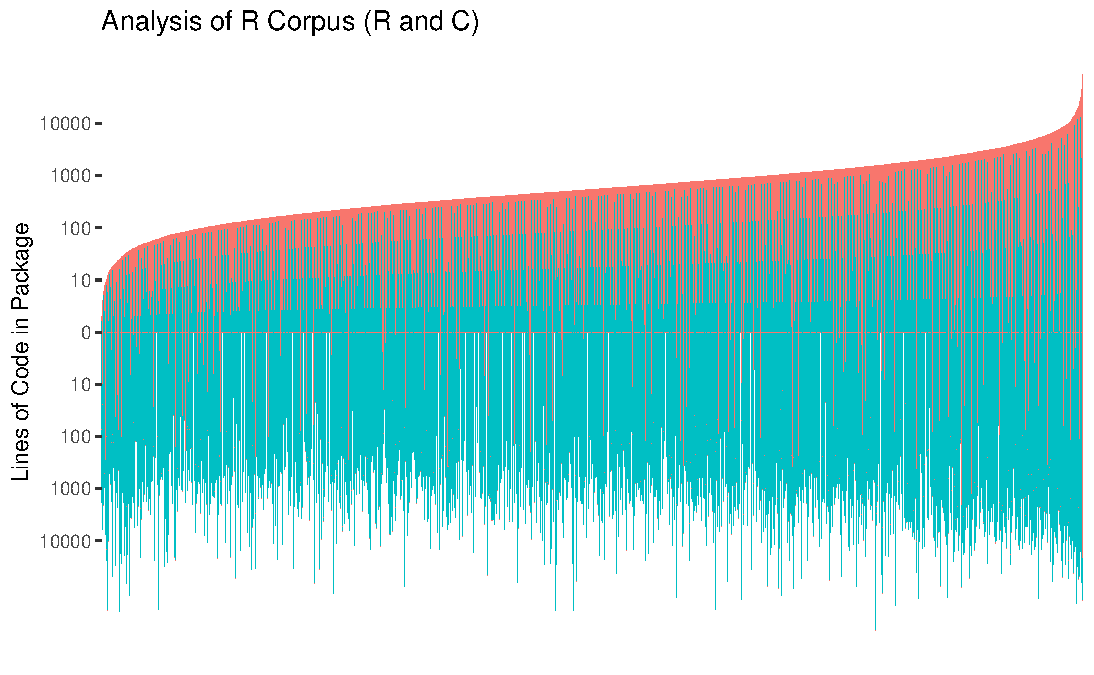
\includegraphics[width=.9\textwidth]{linesofrandccode}
\caption{Lines of code (log scal); for each package, R is above 0, and C/C++
  below}\label{allcloc}\end{center}
\end{figure}


For each package, we extracted all executable code snippets from
documentation, vignettes and tests and ran them independently recording all
calls to R functions.  It is noteworthy that in order to run the scripts in
one package, it is often necessary to load a number of other packages.
In~\cite{issta18}, the authors estimated code coverage to be around 68\%
when including reverse dependencies.  As our infrastructure adds overhead to
script execution, coupled with the fact that some scripts take inordinate
amounts of time to run, this is why we limited our analysis of any given
package to one hour.

% https://www.r-pkg.org/downloaded
\begin{figure}[!th]{\footnotesize\begin{tabular}{@{}r||l|r|r|r|r|r@{}}\hline
\bf Package & \bf Description & \bf R LOC &\bf C LOC &\bf Scripts & \bf Calls Observed & \bf Calls Recorded \\
\hline
\tt Rcpp  & Seamless C++ integration & 2.2K & 4.2K & 25 & 55K & 340 \\
\tt rlang & Functions for 'Tidyverse' & 7.0K & 6.1K & 122 & 3,924K & 8,422 \\
\tt glue  & Interpreted string literals & 0.3K & 0.3K & 8 & 4K & 145 \\
\tt tibble & Simple data frames & 2.0K & 0.3K & 16 & 1,332K & 6,367 \\
\tt stringi &  String processing & 1.5K & 515K & 64 & 923K & 873 \\
\tt ggplot2 & Data visualisations & 14K & 0 & 130 & 153K & 4,608 \\
\tt dplyr  &  Data manipulation & 4.5K & 4.7K & 78 & 233K & 3,099 \\
\tt pillar & Formatting for columns & 1.4K & 0 & 13 & 803K & 1,514 \\
\tt R6 & Classes w. ref. semantics & 0.7K & 0 & 2 & 1K & 330 \\
\tt stringr & String operations & 0.5K & 0 & 32 & 1,764K & 534 \\
\end{tabular}}\caption{10 Most Downloaded Packages.}\label{most}
\end{figure}

Figure~\ref{most} shows the ten most downloaded CRAN packages.  For each
one, we list how many lines of R and C/C++ the packages contains.  We show
the number of scripts that could be extracted from the package. Each script
corresponds to either one use-case or a set of unit tests. We print the
number of function calls that were observed by our infastructure, and the
number of unique signatures that were recorded.

Our infrastructure only retains unique argument/return combinations. Thus,
while we observe large number of functions being called with different
values, the types of these function call are often similar. Over the entire
corpus, we can see the relation between observed and recorded calls in
Figure~\ref{recorded}.  The median number of observed calls is 82 and
maximum is 19 million.  The median number of recorded signatures is 16 and
the maxium is 8,422. These numbers are skewed by a number of scripts doing
very few calls before plunging into C code.

\begin{figure}[htbp]\begin{center}
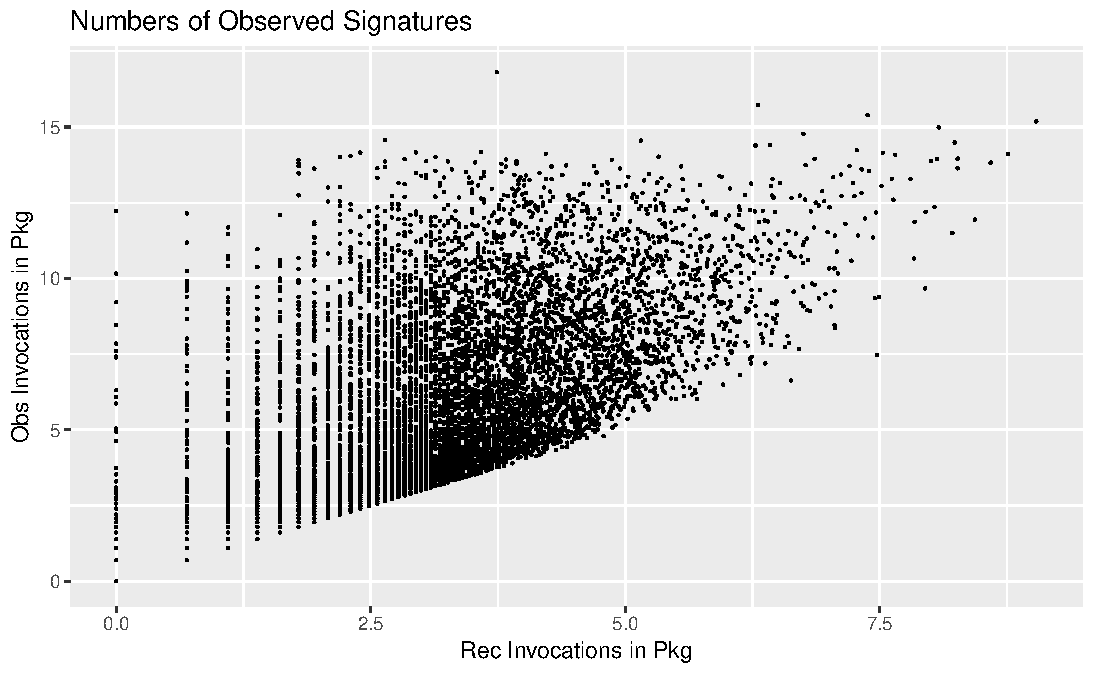
\includegraphics[width=.9\textwidth]{recordsbypkg}
\caption{Numbers of Recorded Function Invocations in the Analyzed Corpus}
\label{recorded}\end{center}
\end{figure}

\newpage
\section{Methods}

In this section, we detail our methodology for collecting data.  Our aim is
to observe arguments and return values of function calls, and from these
generalize possible type signatures for the called functions.  We base our
infrastructure on an open source tool called \genthat whose purpose is to
generate unit tests for R libraries~\cite{issta18}.  \genthat achieves this
by synthesizing unit tests from recorded function argument and return
values, comparing candidate tests against existing ones to avoid generating tests
which do not increase code coverage.  To suit our purposes, we change the
existing tool in two main ways: we record \emph{shapes} rather than values,
and ignore the code coverage optimization phase.  Both changes are
beneficial for scalability, allowing us to trace far more calls.


To illustrate our approach, consider the following script which adds a
double to an integer, and then creates a matrix from a vector, finally
adding them together to get a new matrix.

\begin{figure}[!hb]
\begin{tabular}{ll}\begin{minipage}{5cm}
{\small\begin{lstlisting}[style=R]
> 1 + 2L
[1] 3
> x <- c(1,2,3,4)
> attr(x,"dim") <- c(2,2)
> x + c(1,2)
     [,1] [,2]
[1,]    2    4
[2,]    4    6
\end{lstlisting}}
\end{minipage} &
\begin{minipage}{8cm}\small
\begin{tabular}{rl}
\tt `+`: &\tt \sD \sI \to \sD \\
\tt c:& \sD \sD \sD \sD \to \D\\
\tt `<-`: &\tt \sY \D \to \D\\
\tt c: & \tt \sD \sD \to \D\\
\tt `attr<-`:&\tt  \sY \C \D \to \\
\tt c: &\tt \sD \sD \to \D\\
\tt `+`: &\tt \attr\D{dim} \D \to \attr\D{dim}
\end{tabular}
\end{minipage}
\end{tabular}
\caption{Example script and recorded signature}\label{example}\end{figure}

The functions being called here are \k{`+`}, \k{`<-`}, \k{c} and
\k{`attr<-`}, and the shapes we expect to record are given to the right of the figure.
We abbreviate the types \k{double}, \k{integer}, \k{symbol} and \k{character} to \sD, \sI, \sY, and \sC for simplicity.
\D, \I, \Y, and \C denote vectors, whereas \sD, \sI, \sY, and \sC denote scalars.
We record the lengths of all vectorized-typed values, and for all types we record their classes and attribute names. 
Looking at the signatures observed for addition, it is clear that the function is polymorphic: it starts with the addition of two scalar numbers of different types, and later adds a matrix to a vector returning a matrix.

\subsection{Implementation}
\label{sec:Impl}

A high-level description of the workflow of our tool for one package
retrieved from CRAN is as follows:

\begin{enumerate}
\item {\bf Exec generation:} All runnable code in the package is extracted
  from its tests, examples and vignettes. The code snippets are combined
  into a single file.
\item {\bf Installation:} All packages that are required for execution of
  the current package are downloaded and installed.
\item {\bf Instrumentation:} As code is loaded into the R, every function
  definition is instrumented with an \code{on-exit} hook which is invoked
  when the function returns either normally or through an exception.
\item {\bf Recording:} When a hook is called, arguments and return value are
  inspected. We record \k{typeof}, \k{class} and \k{attributes} recursively.
  For \code{list} values, an extra bit of analysis is performed to record
  the element types.
\item {\bf Writing:} Unique signatures are recorded to file with information
  about which package triggered the recording.
\end{enumerate}

In R, all arguments are passed as promises, and unused arguments will be unevaluated. 
Our recording mechanism captures the order in which arguments are passed, can figure out which arguments were {\it not} provided (recording them as {\it missing} if the missing argument has no default value), and does {\it not} force unforced promises, recording unforced promises as {\it unevaled}.
In R, trying to use missing values results in an error and thus an exception, triggering our recording phase: arguments which cause errors in this way are recorded as {\it error}.
For practical reasons, we do not record the contents of environments:
These can be used as hash tables, may be large, and are quite likely different from one another.

Unevaluated arguments in R are sometimes {\it carefully} used by their functions to implement some form of metaprogramming.
Consider the {\tt magrittr} package, which implements a pipe function \%$>$\% that implements a flavor of function currying:

{\small\begin{lstlisting}[style=R]
mul <- function(x,y)  x*y
4 %>% mul(3)
\end{lstlisting}}

The call to the pipe desugars to \code{`\%>\%`(lhs=4, rhs=mul(3))} where the
\code{rhs} is not a valid expression. It is treated as code that will
manipulated to add one argument (the \code{lhs}), resulting in the function
actually performing a call of the form \code{mul(4, 3)}.

As we alluded to at the beginning of this section, our analysis collects shape information about
arguments and return values in order to be as specific as possible. The details of the information we collect follows.
Note that the first step of any type collection in our analysis begins with \code{typeof}.

\begin{itemize}
\item If the analysis encounters a primitive vector, say
  \code{typeof(x)=="double"}, it records the length of {\tt x} to determine
  if it can be treated as a scalar.
\item For a list, \code{typeof(x)=="list"}, shape information on all
  elements is used to describe the list's shape.  To avoid undue slowdowns,
  we only collect the content's \code{typeof}, and ascribe \ANY (any) if the
  elements are not of the same kind.
\item If the analysis encounters a scalar \code{NA}, we ascribe a unique
  NULL type.  In R, \code{NA} inhabits all types, but for a scalar NA,
  \code{typeof(NA)=="logical"}. Scalar NAs are used as uninitialized values.
\item For a matrix, \code{typeof(m)=="some\_primitive\_type"}, and\code{m} will have matrix class and also a dims and
  optionally dimnames attribute. Here, we ascribe the shape \attr{\tt T}{mat}
  where {\tt T} is the primitive element type.
\item For a data frame, \code{typeof(df)=="list"}, and \code{df} will have class {\tt data.frame}, and {\tt names} and {\tt row.names} attributes.
 To reflect this, we ascribe the shape \attr{\l}{df}.
\end{itemize}

The infrastructure memoizes emitted signatures to avoid writing multiple
identical signatures for the same function.

\section{Types for R}

Our aim is to capture the polymorphism in R, and to do so we must define a meaningful set of basic types for the language.
There are several possible choices, with a variety of levels of expressivity and complexity.
For concreteness, we will pick out three different sets of types.
To start simple, we define a set of types which closely align with R's builtin types, and later define richer notions of type which incorporate attributes, classes, and capture the various object systems of R.

Throughout this paper, we will say that an argument is {\it polymorphic at} \textbf{\emph{LX}} (read: level X) if it has been called with at least two values that belong to distinct types at {\bf LX}.
\textbf{L2} will incorporate class and attribute lists, which are slightly trickier to ``type'', and we defer discussion of this until Section~\ref{sec:L2def}.

\subsection{L0 Types}
\label{sec:L0def}

The logical ``baseline'' for the design of a type system for R is to adopt the language's builtin types.
We dub these {\bf L0} types, and they are primarily built on the \code{typeof} values, which reflects the implementation of the type in the runtime environment.
More specifically, the \code{typeof} a value is simply the runtime type tag of the value.
Given that, {\bf L0} includes the following types: vectors of primitive types (integers
\I, double \D, character \C, logical \L, raw \R, complex \X), lists of any
type (\l), and scalar values (environment \sE, closures \sF, symbols \sY, S4
object \sS, and null \sN). We omit short forms for some of R's more esoteric types (e.g., {\tt environment}s).
 We add the any (written \ANY)  type to stand in for unevaluated values
Subtyping in {\bf L0} follows from the conversion rules of the language:  Logicals are subtypes of integers, which
are themselves subtypes of doubles (so \L <: \I <: \D).  All types are subtypes of \ANY,
thus {\tt T}<:\ANY for an type {\tt T}.

%
%
\subsection{L1 Types}
\label{sec:L1def}

{\bf L0} is limited in expressivity as it (1) supports polymorphism for list in
a trivial way, (2) does not address some of the popular constructed data
types such as matrices and data frames, and (3) cannot differentiate between
scalar values and vectors.  
{\bf L1} types build on and extend {\bf L0} with with scalar values for primitive types (\sI, \sD, \sC, \sL, \sR, and \sX), type-parametric lists (written \lT{T} for any type {\tt T}), data frames (written \attr{\l}{df} as they are built up from lists of type any), and matrices (\attr{\vec{\tt T}}{mat} where {\tt T} is a primitive type).
Subtyping is extended such that {\tt T}<:{$\vec{\tt T}$} for any primitive
type {\tt T}. The subtype relation is undefined for lists of different types, as well as for matrices and data frames.

\subsection{L2 Types}
\label{sec:L2def}

{\bf L2} extends the previous system with support for classes and attributes.
While there are a finite number of results from the \code{typeof} function, this is {\it not} the case for \code{class} and \code{attributes}, as classes and attributes {\it can} be user-defined. 
In terms of classes, R has a number of built-in or otherwise standard classes, ranging from truly primitive classes such as {\tt numeric} to the more complex {\tt data.frame}. 
{\bf L1} already incorporates these builtin classes, namely through its data frame and matrix types, so we will ignore those classes and thus highlight those which are user-defined.  
As for attributes, again some patterns arise naturally in R, e.g. all matrices have a {\tt dims} attribute, but even these are somewhat interesting, as a programmer could in theory set their own {\it dims} attribute on an arbitrary value.
The only attribute we ignore is the {\tt class} attribute, as we collect the class of values separately (and the {\tt class} attribute, if present, is always equal to the class of a value).
Attributes are name-value pairs, and to keep things simple we consider only attribute names.

In sum, we extend {\bf L1} with attribute lists and classes: \attrclass{T}{C}{A} where {\tt T} can be any L1 type other than data frame or matrix, and {\tt C} and {\tt A} are lists of classes and attribute names respectively.  
The subtype relation is defined as: \attrclass{T}{C}{A} $<:_{\mathbf{L2}}$ \xspace \attrclass{\dot T}{C'}{A'} if $ T <:_{\mathbf{L1}} \dot T$ (i.e. are subtypes in the sense of {\bf L1}), $C \subseteq C'$, and $A \subseteq A'$.

Before presenting the results of our analysis, we will quickly survey examples of real, polymorphic R functions that we have analyzed, to build up a global sense of how types manifest themselves in current R code.

%
%
%
%
%
%
\section{Examples of Polymorphism}
\label{sec:polyex}

In this section, we will present an eclectic mix of R functions which exhibit polymorphic behavior at {\bf L0}.

We begin by referring the reader to Figure~\ref{fig:realex}, which showcases the compatibility of integers and doubles.
Coercion from integer to double is performed automatically where appropriate (e.g., here when a double and integer are added together), and likewise coercion from double to integer is automatically performed when integers are strictly required (e.g., here when doubles are being used to index a vector or list).

\begin{figure}[!hb]{\small\begin{lstlisting}[style=R]
> 5L + 1L # => 6L, an integer
> 5L + 1.2 # => 6.2, a double (5L coerced to 5.0)
> c(10, 20, 30)[1.2] # => 10, 1.2 coerced to 1L
\end{lstlisting}}\caption{Example of \sD, \sI type usage.}\label{fig:realex}\end{figure}

Figure~\ref{fig:optnull} shows an example of a function with an optional NULL argument. 
In the function, {\tt x} is a sorted vector of income values, and {\tt w} is a vector of weights with default value NULL.
The function computes fractional ranks required in other package functions.
We see that if {\tt w} is NULL, then default unit weights are generated.
This pattern of default NULL (or NA) arguments is very prevalent in R.

\begin{figure}[!hb]{\small\begin{lstlisting}[style=R]
frac.ranks <- function(x, w=NULL) {
  if (is.null(w)) w <- rep(1, length(x)) # if no weights passed, take all weights = 1
  ...
\end{lstlisting}}\caption{Example of optional argument (from {\tt acid} package).}\label{fig:optnull}\end{figure}

Figure~\ref{fig:listvec} shows an example of a function with list and vector
polymorphism.  The function takes a list or vector {\tt point} and a data
frame {\tt polyg} representing a polygon.  In it, we see that {\tt point} is explicitly converted
to a vector (via the \code{as.numeric} function) regardless of its type.
This showcases the ease with which lists and vectors may be converted in R (the corresponding vector-to-list function is \code{as.list}).

\begin{figure}[!hb]{\small\begin{lstlisting}[style=R]
is.point.inside <- function (point, polyg) {
    p <- as.numeric(point) # as.numeric(list(1, 2)) => c(1, 2)
    ...
\end{lstlisting}}\caption{Example of \l/\D argument (from {\tt bivrp} package).}\label{fig:listvec}\end{figure}

Figure~\ref{fig:charclos} shows an example of a function with character and
function polymorphism.  At a high level, this function
calculates point estimates for an {\tt angmcmc} object (specific to some
packages).  The caller specifies {\tt fn}, which is either a function {\it or} the name of a function which will be evaluated on the object samples to estimate parameters.
If {\tt fn} is a string, the function lookup is performed by \code{match.fun}.

\begin{figure}[!hb]{\small\begin{lstlisting}[style=R]
pointest <- function (object, fn = mean, par.name, comp.label, chain.no,  ...) {
    ...
    if (is.character(fn))
        if (fn == "MODE" | fn == "MAP")   do_MAP <- TRUE
        else {
            do_MAP <- FALSE
            fn <- match.fun(fn) # looks up the function name
        }
\end{lstlisting}}\caption{Example of \sC/\sF argument (from {\tt BAMBI} package).}\label{fig:charclos}\end{figure}

In Figure~\ref{fig:dfdbl}, we see a function that, among other things, takes in some data ({\tt dat}) and a
character string ({\tt spss}) specifying either {\tt "in"} or {\tt "out"}.
Here, the type of {\tt dat} is {\it dependent} on the value of {\tt spss}:
if {\tt spss == "in"}, {\tt dat} must be a data frame, and otherwise if {\tt spss == "out"}, {\tt dat} must be a vector.
Our analysis does not capture this granularity of dependency, as we only collect type information.

\begin{figure}[!hb]{\small\begin{lstlisting}[style=R]
nret.translator <- function(dat, spss="out", ...) {
  ...
  if(identical(spss, "out")) {
    if(!is.vector(dat))  stop(simpleError("...'dat' must be a vector!"))
    ...
  } else {
    ...
    # here, dat is data.frame
    items.idx <- items.idx[order(names(dat[, items.idx]))]
  }
\end{lstlisting}}\caption{Example of a \df/\D argument (from {\tt klausR} package).}\label{fig:dfdbl}\end{figure}

In Figure~\ref{fig:chardbl}, we see a function which takes in a list ({\tt network}), a vector of indices of that list ({\tt fixIndices}), and a
vector of values ({\tt values}).  The locations specified by {\tt fixIndicies} in {\tt network} are updated with {\tt values}.  Here, {\tt fixIndicies} has been observed to be either a character or double vector:
In R, list indices are typically doubles, but can be characters (if the list
or vector being indexed has a {\tt names} attribute).
Note that type level {\bf L2} can capture the presence of a {\tt names} attribute.

\begin{figure}[!hb]{\small\begin{lstlisting}[style=R]
fixGenes <- function (network, fixIndices, values) {
  ...
  network$fixed[fixIndices] <- as.integer(values)
  ...
\end{lstlisting}}\caption{Example of \C/\D argument (from {\tt BoolNet} package).}\label{fig:chardbl}\end{figure}

In Figure~\ref{fig:matvec}, we see that a function which can take in a vector,
but immediately transforms it (transpose, with {\tt t}) into a matrix.  As
an idea, matrix/vector polymorphism seems sensible, as mathematically
vectors {\it are} one-dimensional matrices.  R echoes this by making conversion between the two
types easy: \code{as.vector(m)} flattens a matrix \code{m} into a vector
(e.g., \code{as.vector(matrix(2, 2, 2)) == c(2, 2, 2, 2)}), and
\code{as.matrix(v)} builds a {\tt length(v) x 1} matrix (e.g.,
\code{as.matrix(c(1, 2)) == matrix(data=c(1, 2))}).  \AT{TODO fix line break
  in code at end of last sentence}
  
\begin{figure}[!hb]{\small\begin{lstlisting}[style=R]
tee <- function (x, theta, D1, D2, phi)  {
    if (is.vector(x)) x <- t(x)
    ...
\end{lstlisting}}\caption{Example of matrix/(\D) argument (from {\tt calibrator} package).}\label{fig:matvec}\end{figure}

Throughout this short section, we have shown real examples of polymorphic R functions.
Our goal is to capture these instances of polymorphism across a large subset of existing R code, and to highlight and discuss patterns which arise.
We present the results of our analysis in the following section.

%
%
%
%
%
%
\section{Analysis Results}\label{sec:results}

This section presents our results for each of the levels we have considered.
\AT{New numbers will be available tonight (Apr 5).}
\AT{Will use that to fill in some blanks.}

\subsection{L0}

At {\bf L0}, the type system is mostly aligned with the types of the core language.  We
have observed over \AT{how many?} monomorphic functions; this accounts for \AT{what \%?} of our
corpus. 

Across all of the arguments that we've observed, the vast majority are monomorphic.
Table~\ref{tab:L0top10arg} shows the breakdown of the 10 most frequently occurring argument signatures.
\begin{table}[ht]
\label{tab:L0top10arg}
\centering
\begin{tabular}{lrr}
  \hline
 Argument Signature & Count & Percentage \\ 
  \hline
  \D & 69806 & 26.3\% \\ 
  \l\ & 55311 & 20.8\% \\ 
  \C & 27789 & 10.5\% \\ 
  \L & 26230 & 9.9\% \\ 
  \sF & 16806 & 6.3\% \\ 
  \sN & 13976 & 5.3\% \\ 
  \ANY & 9125 & 3.4\% \\ 
  \I & 8971 & 3.4\% \\ 
  \sS & 4748 & 1.8\% \\ 
  \D, \I & 3256 & 1.2\% \\ 
   \hline
\end{tabular}
\caption{Most frequent argument signatures in {\bf L0}.}
\end{table}

We see that doubles are the most common argument type, which is not entirely surprising as doubles are the backbone of any numeric data.
Next is lists, which seems reasonable given that lists are often used to store the aforementioned data.
Recall that in {\bf L0}, data frames will appear as lists.
The \ANY type is not an R type per se: we ascribe such a type to arguments which were {\it always} unevaluated across all calls.
As it happens, many R functions metaprogram on some of their arguments, and this metaprogramming does not force the argument promise, and if this metaprogramming is always performed in every recorded call we will ascribe the \ANY type, as we cannot say what the argument {\it is} without possibly forcing a promise.
The magrittr package's pipe \%$>$\% function is an example of a function which performs a lot of metaprogramming; we will discuss it in a little more detail shortly.

One of our chief goals is to generate useful function signatures.
After tracing and capturing unique signatures from function call sites, \AT{recall} that we collapse some of the more obvious ones together.
After this, we are curious to know: {\it how many functions have more than one signature?}
Figure~\ref{fig:L0funcounts} has the answer with a breakdown by function.

\begin{figure}[htbp]\begin{center}
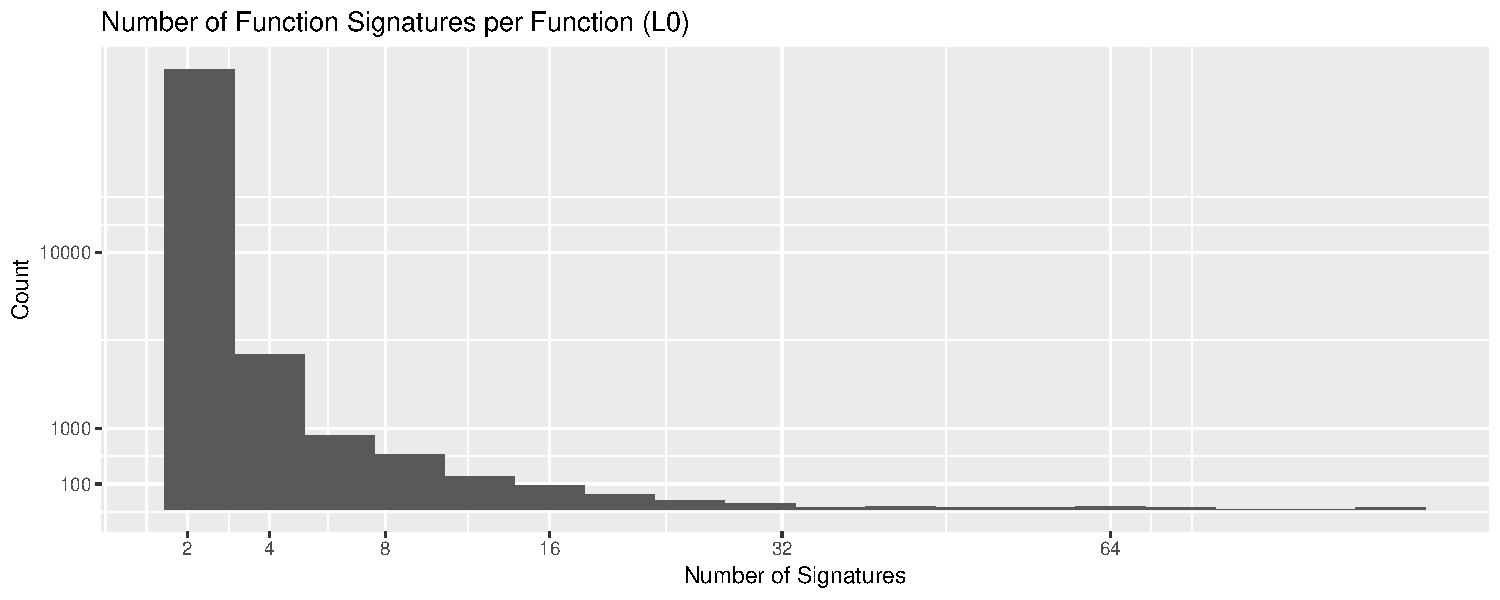
\includegraphics[width=.9\textwidth]{L0_by_fun}
\caption{Record of Function Polymorphism in {\bf L0}. \LZEROPERCPOLY of functions are polymorphic.}
\label{fig:L0funcounts}\end{center}
\end{figure}

Here, we see that the vast majority of functions are monomorphic in L0.
That said, there are a few functions with a disproportionately large number of signatures.
One such function is the magrittr package's pipe \%$>$\%, which is used to implement a kind of currying (as per discussion in Section~\ref{sec:Impl}).
Many of the metaprogramming functions in the Tidyverse are quite sophisticated, and are designed with the explicit goal of being very usable.
This usability maps to polymorphism in our analysis, so it's no surprise that a Tidyverse function features so prominently here.

Another function with many signatures is the data.table package's [ function, which is overloaded for objects with data.table class.
This function has 16 formal arguments, and call configurations vary widely.
Essentially, [ is {\it the} main function for data.tables, and performs very different tasks based on which arguments are provided.
Two wildly different uses are:
\code{DT[i, j, by]}, where columns \code{i} and \code{j} are accessed and grouped by \code{by}, and \code{DT[x == "some" & y > 42]}, which selects all rows who's \code{x} column is the string \code{"some"} and who's \code{y} column is greater than \code{42}.
Given that, we find it unsurprising that the function is so polymorphic.

In choosing how to express the polymorphicity of a function, there are two main options one might consider:
First, having several separate whole-function signatures, e.g. \D $\rightarrow$ \D and \C $\rightarrow$ \D, or alternatively expressing the polymorphism at the argument level with a union type, e.g. (\D $\cup$ \C) $\rightarrow$ \C.
The former is referred to as {\it per-function} or {\it function-level polymorphism}, and the latter as {\it per-argument} or {\it argument-level polymorphism}.
Earlier in Table~\ref{tab:L0top10arg} we saw the most frequently occurring argument-level signatures, and Figure~\ref{fig:L0funcounts} broke our corpus down by function-level polymorphism.

To get an idea of the most common forms of argument-level polymorphism, we refer toTable~\ref{tab:L0toppoly}.

\begin{table}[ht]\label{tab:L0toppoly}\centering
\begin{tabular}{lrr}  \hline
Signature & Count & \% of All Signatures \\
\hline
  \D, \l & 2799 & 1\% \\ 
  \D, \sN & 2290 & 0.9\% \\ 
  \C, \sN & 1527 & 0.6\% \\ 
  \l, \sN & 1193 & 0.4\% \\ 
  \C, \D & 858 & 0.3\% \\ 
  \D, \sF & 413 & 0.2\% \\ 
  \C, \I & 382 & 0.1\% \\ 
  \I, \sN & 378 & 0.1\% \\ 
  \C, \l & 371 & 0.1\% \\ 
  \C, \sF & 334 & 0.1\% \\ 
\end{tabular}
\caption{Top polymorphic argument signatures for the L0 type system.}
\end{table}

Let's unpack some of the signatures in Table~\ref{tab:L0toppoly}:

\begin{itemize}

	\item \D, \l (and \C, \l): L0 doesn't parameterize list types, and it's very likely that this signature describes vectors of doubles and lists of doubles.
	Coercing vectors to lists is trivial in R, and indeed many of the functions with such an argument signature do.
	The story is similar with vectors of characters and lists of characters.
	
	\item $\square$, \sN: there are a few instances of this ``null'' polymorphism.
	The frequency of these signatures indicates a tendency to create ``optional arguments'', where some argument's default value might be NULL.
	This pattern is quite frequent in R code, and an example can be found in Figure~\ref{fig:optnull}.

	\item \C, \D and \C, \I: these are interesting patterns.
	In R, lists can always be indexed with numerics (\L, \D, \I) {\it and also} characters.
	When a list is indexed by character, the character is matched against the element names in the list and the corresponding element is selected.
	If there is no match, the lookup returns NULL.
	Another possible explanation for these signatures are dates, which can be represented by numerics or characters and the value usually has one of the date classes.
	L0 doesn't deal with classes, which are one of the topics of L2.

	\item \D, \sF: this signature appears more strange than it is.
	Many models, processes, simulations, etc. that are prevalent throughout R are are {\it parameterized}.
	Some arguments with the \D, \sF signature are either parameters for a function (\D), or the function itself already constructed (\sF).
	Others, such as the {\tt br} argument of the {\tt rtree} function in the {\tt ape} package, are either parameters for complex data generation processes (\D), or a function to be used during the generation (\sF).
	It would appear that this pattern is used to make complex simulation, modelling, or data generation functions more flexible for programmers.
	
	\item \C, \sF: yet another puzzling signature, though its explanation is surprisingly straightforward:
	In R, programmers are free to look functions up {\it by name}, and indeed the frequently encountered {\tt UseMethod} function for dynamic class-based function dispatch is one such example.
	In short, this signature usually represents a function or a function name.

\end{itemize}

We have established and discussed some of the most common polymorphic attribute signatures, and have built up an understanding of argument-level polymorphism in the {\bf L0} type system.
This matches almost exactly with the language as it is today, as {\bf L0} is in (nearly) 1:1 correspondence with how types are currently represented in the language.
The next question we address is: {\it just how pervasive is this argument polymorphism?}
Refer to Table~\ref{tab:L0argcounts}.

\begin{table}[ht]\label{tab:L0argcounts}\centering
\begin{tabular}{lrl}
  \hline
Signature Type & Count & Percentage \\ 
  \hline
  Monomorphic & 250K & 94\% \\ 
  Total Seen & 266K & --- \\ 
   \hline
\end{tabular}
\caption{Argument position polymorphism in L0.}
\end{table}

From Table~\ref{tab:L0argcounts} we see that, with our definition of subtyping on L0 and other simplifications we made, an overwhelming amount of argument polymorphism is accounted for.
We also saw in Table~\ref{tab:L0toppoly} that each of the most frequently occurring argument signatures had some explanation.
That said, L0 is not without limitations.

The main issues with L0 stem from a lack of adequate information, as the type system doesn't capture precise list types, and does not distinguish scalars from vectors.
The next type system we will explore, L1, tackles these issues by collecting more information to build more precise types.
While the L1 types are less ``in-tune'' with current R implementations, one can imagine designing an all-new R runtime which may benefit from the more specific information in L1, e.g. by not needing to vectorize scalar values, or designing a static analysis which uses precise list types to give programmers better information in an IDE.
L1 is discussed next.

\AT{TODO do function signatures maybe? Maybe just an example that we can run with.
Plots also.}

%
%
%
%
\subsection{L1}

As we mentioned in Section~\ref{sec:L1def}, L0 is somewhat limited in its expressivity. 
To address this, we develop L1, which espouses a finer-grained approach to types. 
Major modifications from L0 include:

\begin{enumerate}
	\item the differentiation of scalars and vectors;
	\item the parameterization of list types over element types;
	\item the use of attribute and class information to distinguish types for data frames and matrices, and;
	\item subtyping of \sN (i.e., $\forall T$, \sN $<:$ $T$).
\end{enumerate}

An example of a signature in this type system can be found in
Figure~\ref{fig:exL1}.

\begin{figure}[!hb]{\small\begin{lstlisting}[style=R]
add_make_list <- function(x, y) {
  l <- as.list(x + y)
  attr(l, "example") <- "this is an attribute"
  l
}
add_make_list(2, c(3, 1)) # => list(5, 3)
\end{lstlisting}}
\caption{Call signature in L1: x: \sD, y: \D $\rightarrow$ \lT{D}.}\label{fig:exL1}\end{figure}

Let us begin as we did in L0 by looking at the breakdown of argument signatures in L1.
Consult Table~\ref{tab:L1top10arg}.
\begin{table}[ht]
\label{tab:L1top10arg}
\centering
\begin{tabular}{lrr}
  \hline
 Argument Signature & Count & Percentage \\ 
  \hline
  \sD & 48815 & 18.4\% \\ 
  \D & 27367 & 10.3\% \\ 
  \sL & 24284 & 9.2\% \\ 
  \sC & 22025 & 8.3\% \\ 
  \l & 20062 & 7.6\% \\ 
  \sF & 18480 & 7\% \\ 
  \M{D} & 14315 & 5.4\% \\ 
  \sN & 14016 & 5.3\% \\ 
  \ANY & 9093 & 3.4\% \\ 
  \C & 7731 & 2.9\% \\
   \hline
\end{tabular}
\caption{Most frequent argument signatures in L1.}
\end{table}

From Table~\ref{tab:L1top10arg}, we see that all of the most frequent argument signatures are monomorphic even though we increased the precision of the types.
We see that scalars actually figure quite prominently, which is encouraging, supporting our suggestion of an explicit scalar annotation.
We also see that matrices (\M{D}) are quite popular, a testament to the versatility of the data structure, as they can easily be converted to vectors and data frames.

Now that we have a picture of how arguments look in L1, let's see: {\it how many L1 functions have more than one type signature?}
The answer can be found in Figure~\ref{fig:L1funcounts}.

\begin{figure}[htbp]\begin{center}
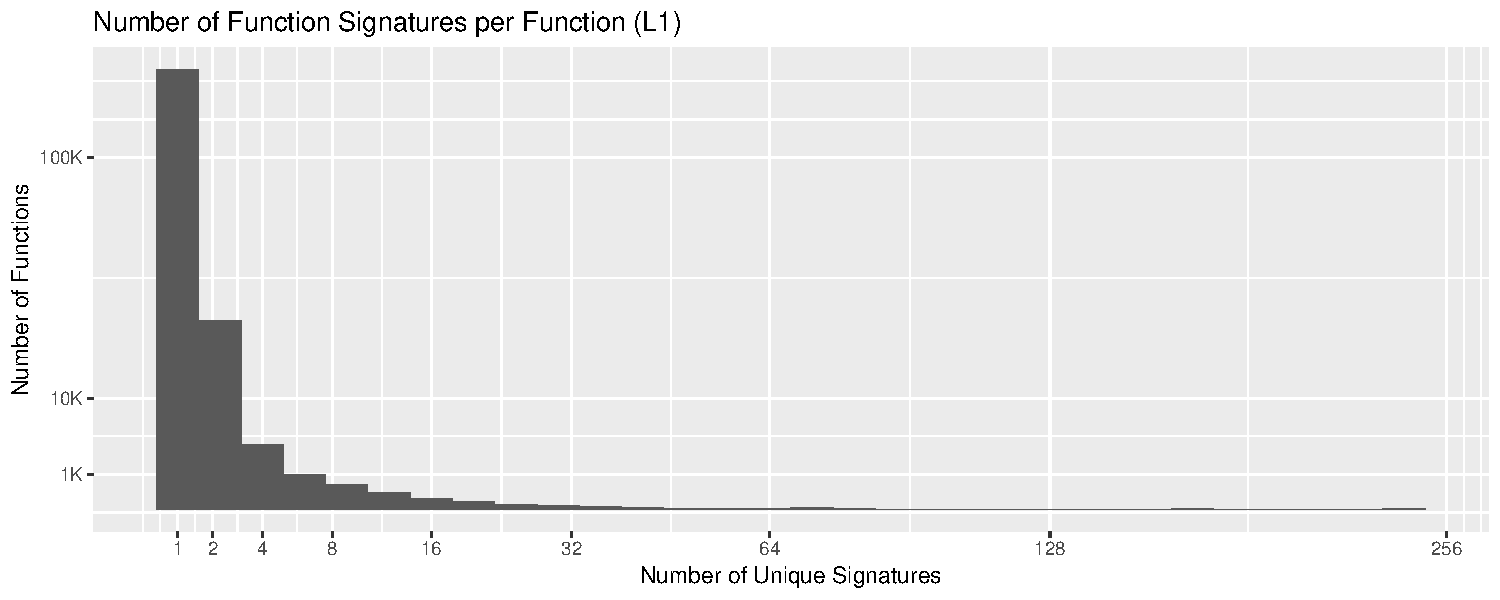
\includegraphics[width=.9\textwidth]{L1_by_fun}
\caption{Record of Function Polymorphism in {\bf L1}. \LONEPERCPOLY of functions are polymorphic.}
\label{fig:L1funcounts}\end{center}
\end{figure}

We see that we increased the polymorphism with our transition to L1, despite the monomorphic nature of the most frequently appearing argument signatures.
As we were in L0, we are curious to know how argument-level polymorphism looks in L1.
Refer to Table~\ref{tab:toppolyL1}.

\begin{table}[ht]
\label{tab:toppolyL1}
\centering
\begin{tabular}{lrl}
  \hline
Signature & Count & \% of All Signatures \\ 
  \hline
  \D, \M{D} & 1440 & 0.5\% \\ 
  \l, \lT{D} & 525 & 0.2\% \\ 
  \M{D}, \M{I} & 383 & 0.1\% \\ 
  \sC, \sD & 382 & 0.1\% \\ 
  \I, \sD & 370 & 0.1\% \\ 
  \l, \lT{list} & 337 & 0.1\% \\ 
  \df, \M{D} & 305 & 0.1\% \\ 
  \C, \D & 294 & 0.1\% \\ 
  \sD, \sF & 290 & 0.1\% \\ 
  \sC, \sF & 273 & 0.1\% \\
   \hline
\end{tabular}
\caption{Top polymorphic argument signatures in L1.}
\end{table}

So what do these signatures mean?

\begin{itemize}
	\item \D, \M{D}: vectors are just one-dimensional matrices.
	Indeed, the only thing separating a vector from a matrix in R is a {\tt dims} attribute.
	
	\item \l, \lT{D}: this hearkens back to L0, where we discussed how this very same signature was explained by the list being a list of doubles.
	So why is it still here?
	Well, first note that there are far less of these signatures in L1 than in L0, so clearly we captured {\it something}.
	Next, note the method with which we parameterize lists: we ascribe some type $T$ to a list type \lT{T} if and only if {\it all} list elements have {\it exactly} type {\it T}---in our analysis, we have encountered lists with integers as well as doubles, and unfortunately those currently appear as \l.
	This could be addressed by doing some subtyping computation while exploring list elements.
	
	\item \M{D}, \M{I}: this signature is reasonable, as any computation in R on \M{D} would work on \M{I} and vice versa.
	
	\item \sC, \sD and \C, \D: we discussed this in L0---this signature likely captures an index or a date.
	
	\item \I, \sD: subtyping between primitives does not hold between scalars and vectors (i.e., \I $\not<:$ \sD) even though it's likely that the programmer intended for the argument to be a vector of the supertype (here, these arguments were likely intended to be of type \D).

	\item \l, \lT{list}: here we have a list of any and a list of lists.
	One explanation for this is that lists of lists sometimes contain NULL as an element, and this would show up with type \l, again as we don't do any subtyping while computing precise list types.
	Another explanation is the way R handles object-orientation, which we discuss shortly in Section~\ref{sec:S3S4R5}.
	
	\item \df, \M{D}: in R, it's easy to transform a matrix into a data frame, and this argument is likely a result of that:
	Simply calling \code{as.data.frame} on a matrix is enough.
	
	\item \sD, \sF and \sC, \sF: these were thoroughly discussed in the context of L0.
	
\end{itemize}

With an understanding of argument polymorphism in L1, we wonder: {\it how many argument positions are polymorphic in L1?}
Refer to Table~\ref{tab:argcountsL1}.

\begin{table}[ht]
\label{tab:argcountsL1}
\centering
\begin{tabular}{lrl}
  \hline
Signature Type & Count & Percentage \\ 
  \hline
  Monomorphic & 252K & 94.9\% \\ 
  Total Seen & 265K & --- \\ 
   \hline
\end{tabular}
\caption{Argument position polymorphism in L1.}
\end{table}

In spite of drastically increasing the precision of our types, we are still happily only dealing with a small amount of polymorphism.
This suggests that with a good notion of subtyping, precise type annotations won't cause an undue increase in the polymorphism of the language.

Before presenting L2, we will digress slightly and explore some of the ramifications of our transition from L0 to L1.

%
%
\subsubsection{Scalars}
\label{sec:scalars}

Our suggestion to add an explicit scalar type is not unfounded, though it is not compatible with current R implementations.
We saw in this section that strictly scalar values appear quite frequently, making up some of the most frequently occurring argument signatures.
In fact, \PERCSCALARMONO of arguments have a strictly scalar monomorphic signature.
This suggests that such a distinction would more accurately capture current use of the language, and would also be beneficial to future implementations which can perform optimizations based on the type (e.g., not vectorizing scalar-only values).

%
%
\subsubsection{Object-Oriented Programming in R}
\label{sec:S3S4R5}

There is something more to be said about the \l type, namely that it is sometimes linked to (one of) R's takes on object-oriented programming.
R has three object systems: S3, S4, and R5, and S3 objects will often manifest themselves with this signatures in L1.
An S3 object is any value with a ``class'' attribute, and indeed many of these tend to be lists.
For example, an S3-style ``Point'' might be a list with an entry for each dimension in the point, with a ``class'' attribute set to ``Point''.
When these S3 objects have contents with a variety of types, their L1 type will appear as \l, which leaves something to be desired:
Our next type system, L2, will remedy this.

%
%
\subsubsection{\C, \I, \D Polymorphism}
Another significant source of apparently strange polymorphism is the character, integer, double polymorphism.
Figure~\ref{fig:chardbl} lays out an example of this polymorphic signature, showing that lists and vectors can be accessed by strings as well as numerics.
One could conceive of an ``index'' type to capture this, but there are certain limitations to such a type, as such an ``index'' cannot be incremented as it could be a string.
An even more sophisticated dependent type system could capture this, but it's far from clear if such a sophisticated type system would be for a language like R.

One other possible explanation for this polymorphism is the ``date'' data type.
In R, dates are often represented as either strings or numbers, and they are widely used.
Dates (sometimes) manifest themselves in the class of a value, for examples refer to Figure~\ref{fig:date}.
\begin{figure}[!hb]{\small\begin{lstlisting}[style=R]
class(date()) # => character
class(Sys.Date()) # => Date
class(as.POSIXlt(Sys.Date())) # => POSIXlt, POSIXt
as.integer(as.Date(1, origin = "1900-01-01"))
\end{lstlisting}}\caption{Dates in R.}\label{fig:date}\end{figure}

Unfortunately, the format of dates in R is not standardized.
That said, translating between date representations is straightforward.
As most dates are classes, L2 will be able to capture their use.

Throughout this section, we have seen that even though we substantially increased the precision of our type annotations, we have not increased the amount of polymorphism that we observe.
The transition from L0 to L1 revealed some interesting patterns that L1 cannot quite capture---for these, we will need to appeal to the class and attributes of values.
The next type system we consider is L2, and is designed to achieve this.

%
%
%
%
\subsection{L2}

{\bf L2} works class and attribute information into its type signatures.
As per the discussion in Section~\ref{sec:L2def}, we omit builtin classes in order to highlight those which are user-defined.
{\bf L2} differs from {\bf L1} in the following ways:

\begin{enumerate}

	\item where {\bf L1} and {\bf L0} only considered classes and attributes when ascribing matrix or data frame types, {\bf L2} considers classes and attributes to be an integral part of the type system.
	Annotations in {\bf L2} include classes and attribute names when they are present.
	
	\item recall that subtyping between two {\bf L2} types is defined as 
	
\end{enumerate}

As in {\bf L0} and {\bf L1}, we will begin by showing a breakdown of the top argument signatures in Table~\ref{tab:L2top10arg}.

\begin{table}[ht]
\label{tab:L2top10arg}
\centering
\begin{tabular}{lrl}
  \hline
Signature & Count & \% of All Signatures \\ 
  \hline
  \sD & 46938 & 17.6\% \\ 
  \sL & 24113 & 9\% \\ 
  \sC & 21387 & 8\% \\ 
  \D & 20900 & 7.8\% \\ 
  \sF & 14556 & 5.5\% \\ 
  \sN & 14016 & 5.3\% \\ 
  \ANY & 9093 & 3.4\% \\ 
  \attrclass{\D}{}{dim} & 6974 & 2.5\% \\ 
  \C& 6939 & 2.6\% \\ 
  \attrclass{\l}{}{names} & 6137 & 2.2\% \\ 
   \hline
\end{tabular}
\caption{Most frequent argument signatures in {\bf L2}.}
\end{table}

As you can see, the most frequent signatures in {\bf L1} are represented here.
The inclusion of class and attribute information has changed the counts slightly.
One tidbit of interest here is that monomorphic named lists are more common than their unnamed counterparts.
The lack of classes is explained by our elimination of builtin classes, and it's doubtful that a user-defined class would be so pervasive as to feature in this breakdown.

Now that we have a sense for argument-level type signatures in {\bf L2}, we will see just how many functions are polymorphic.
Now, {\bf L2} builds directly off of {\bf L1}, and as such at the argument level the type-based polymorphism shouldn't change.
For this account of polymorphism, we deem an argument to be polymorphic if it was polymorphic in type, class, or attribute pattern.
Consider Figure~\ref{fig:L2funcounts}.

\begin{figure}[htbp]\begin{center}
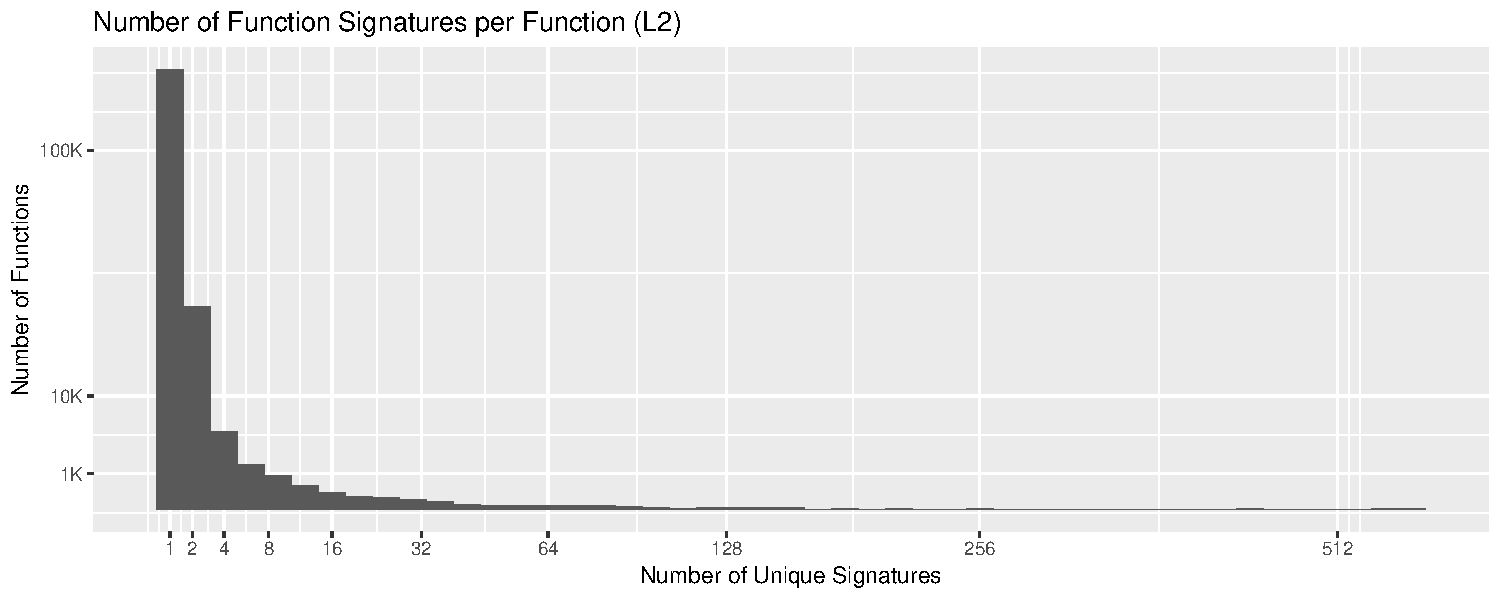
\includegraphics[width=.9\textwidth]{L2_by_fun}
\caption{Record of Function Polymorphism in {\bf L2}. \LTWOPERCPOLY of functions are polymorphic.}
\label{fig:L2funcounts}\end{center}
\end{figure}



Having built a sense for how polymorphic whole-function signatures are in {\bf L2}, we will turn our attention to polymorphic arguments.
Given the added class and attribute information, {\it what do the more frequent polymorphic argument signatures look like?}
Table~\ref{tab:toppolyL2} has the breakdown.

% latex table generated in R 3.5.1 by xtable 1.8-3 package
% Fri Apr  5 09:50:59 2019
\begin{table}[ht]
\label{tab:toppolyL2}
\centering
\begin{tabular}{lrl}
  \hline
Signature & Count & \% of All Signatures \\ 
  \hline
  \D, \attrclass{\D}{}{dim} & 553 & 0.2\% \\ 
  \sC, \sD & 336 & 0.1\% \\ 
  \I, \sD & 320 & 0.1\% \\ 
  \attrclass{\l}{}{names}, \attrclass{\D}{}{names} & 269 & 0.1\% \\ 
  \D, \attrclass{\D}{}{dim, dimnames} & 218 & 0\% \\ 
  \sD, \sF & 173 & 0\% \\ 
  \attrclass{\l}{}{names, row.names}, \attrclass{\D}{}{dim, dimnames} & 167 & 0\% \\ 
  \attrclass{\D}{}{names}, \attrclass{\D}{}{dim, dimnames} & 155 & 0\% \\ 
  \C, \I & 149 & 0\% \\ 
   \hline
\end{tabular}
\caption{Top polymorphic argument signatures in {\bf L2}.}
\end{table}

\AT{Will have new numbers by tonight.}

When comparing this table with Table~\ref{tab:toppolyL1}, we see that the distribution of signature frequencies is more uniform, as attributes and classes differentiated some signatures which were not distinct in {\bf L1}.

Now that we have seen the most frequently appearing argument signatures, we ask: {\it how many argument positions are polymorphic?}.
Table~\ref{tbl:argcountsL2} has the answer.

\begin{table}[ht]
\label{tab:argcountsL2}
\centering
\begin{tabular}{lll}
  \hline
Signature Type & Count & Percentage \\ 
  \hline
  Monomorphic & 248K & 93.4\% \\ 
  Total Seen & 265K & --- \\ 
   \hline
\end{tabular}
\caption{Account of {\it argument} polymorphism in {\bf L2}.}
\end{table}

Surprisingly, even with the added precision of classes and attributes, there is still a relatively small amount of argument-level polymorphism in {\bf L2}.
Our notion of subtyping on classes is rather weak, and one extension would be to include class hierarchies in the subtyping of classes;
this would further reduce the amount of polymorphism in this type system.



%
%
%
%
\subsection{Notable Patterns and Observations}

Besides exploring the patterns highlighted by our various type systems, we can address some interesting and tangentially related questions about the usage of types in R.

%
%
%
%
\subsubsection{R's Most Polymorphic Functions}

Given the data that we've collected, it's natural to wonder what the most polymorphic packages are.
Indeed, we have shed some light on some of the most polymorphic {\it functions}, but what about the packages that these functions belong to?
What is their purpose, and why are they so polymorphic?
Figure~\ref{tab:packagepolysize} has some answers.
Note that we are in the context of {\bf L0}, here, to highlight current language patterns.

% latex table generated in R 3.5.1 by xtable 1.8-3 package
% Thu Mar 28 18:15:26 2019
\begin{table}[ht]
\label{tab:packagepolysize}
\centering
\begin{tabular}{lrrr}
  \hline
  Package & \# of Functions &\# of Signatures & Description \\ 
  \hline
  knitLatex & 4 & 41 & \LaTeX \xspace generator from R data \\ 
  magrittr & 17 & 126 & Tidyverse pipe suite \\ 
  proto & 5 & 30 & Prototype object-based programming \\ 
  gnlm & 10 & 53 & Regression fit package \\ 
  Formula & 17 & 82 & ?? \\ 
   \hline
\end{tabular}
\caption{5 most polymorphic packages (in {\bf L0}).}
\end{table}

Now, what makes these so polymorphic?

\AT{TODO if time: fix to score per fun, then tally per package.}

\begin{enumerate}

	\item knitLatex: two functions are largely responsible for this level of polymorphism: sTab, which produces \LaTeX \xspace supertabular environments, and lTab, which produces \LaTeX \xspace longtable environments.
	These functions both have over 15 arguments, and there are a large number of recorded configurations, with many of the arguments being optional.
	
	\item magrittr: we discussed magrittr earlier in the context of its pipe \%$>$\% function. 
	It's not surprising that the package as a whole is quite polymorphic, as it implements {\it several} different pipe functions, e.g. \%$<>$\% which pipes as normal and then assigns to the left-hand argument.
	
	\item proto: most of the polymorphism in this package comes from its implementation of assignment ({\tt \$<-}) for proto class objects.
	It's a small, 3 argument function which is exceedingly polymorphic, with over 20 unique call signatures.
	As theoretically any R object can have a proto class, it stands to reason that this function ought to be quite polymorphic indeed.
	
	\item 
	
	\item 

\end{enumerate}

It's highly improbable that a static type system designed for an untyped language will be able to capture all of the language's existing code (without resorting to an \ANY type or abusing unions).
It's also unclear how useful a type system would be if it {\it did} capture everything.
Indeed, many of the packages discussed here are really designed to take in anything for particular arguments (e.g., left-hand side of \%$>$\%), and restricting these functions should not be the goal of any static type system designed after a language has matured.

%  magrittr & 4.16 &  \\
%  types & 3.25 & Simple type annotations for R \\
%  r6extended & 3.00 & Utilities extending barebones R6 package \\
%  utils & 2.93 & Utilities for R developers \\
%  zeallot & 2.85 & Metaprogramming package for assignment \\
%  listviewer & 2.72 & R list visualizer \\
%  proto & 2.60 &  \\
%  apercu & 2.49 & Display a short view of a complex R value (list, vector, etc.) \\
%  pipeR & 2.46 & Another pipe suite \\
%  rethinker & 2.44 & RethinkDB client for R \\

%% latex table generated in R 3.5.1 by xtable 1.8-3 package
%% Thu Mar 28 16:01:37 2019
%\begin{table}[ht]
%\label{tab:bigpolyfuns}
%\centering
%\begin{tabular}{llrl}
%  \hline
%Package & Function & Size & Description \\
%  \hline
%  magrittr & \%$>$\% & 23.00 & Tidyverse pipe function \\
%  magrittr & freduce & 17.67 & Apply a list of functions sequentially \\
%  rlang & captureArgInfo & 16.50 & Capture arg info \\
%  rlang & enquo & 16.00 & Create quosure \\
%  rlang & get\_expr & 15.00 & Extract expression \\
%  data.table & replace\_dot\_alias & 13.50 & Deals with '.' in passed expr \\
%  tibble & strip\_dim & 13.00 & Removes 'dim' attribute \\
%  data.table & copy & 11.00 & Create copy of passed value \\
%  htmlwidgets & shouldEval & 11.00 & Eval passed value depending on tag \\
%  magrittr & \%$<$$>$\% & 11.00 & Like \%$>$\% but assigns \\
%   \hline
%\end{tabular}
%\caption{10 most polymorphic functions.}
%\end{table}

%
%
%
%
\subsubsection{Metaprogramming and Unevaluated Arguments}

Our analysis uncovered a non-negligible amount of argument positions which were {\it never} evaluated across all observed function calls.
This is indicative of a desire to metaprogram arguments and otherwise deconstruct their AST, as the \%$>$\% function does.
This is an incredibly powerful language feature, and may well be at the source of R's popularity, if in a roundabout way.
Tidyverse, by far the most popular package suite in R, owes some of its success to the new syntax defined by some of the included packages, and it's this ability to metaprogram arguments which allowed Tidyverse to define its unique syntax.
An example of that syntax is \%$>$\%, and indeed this function was highly exercised by over 100 other packages.

%
%
%
%
%
%
\section{Discussion}

\AT{Short section to recap the analysis results, discuss trends, consolidate our suggestions, talk about argument vs. function poly.}

%
%
%
%
\subsection{Function Polymorphism}

\AT{Retool this into possible meta discussion after results}

Now, we will turn our attention to whole function polymorphism.

This is different because we can now look at argument polymorphism across several arguments, like we did when thinking about character/real polymorphism.

We're interested to see what kinds of ``meta-annotations'' we can make at the function level.
For instance, should we link argument types with return types?
Consider Figure~\ref{fig:funanno}.
\begin{figure}[!hb]{\small\begin{lstlisting}[style=R]
iden <- function(x) x;

# observed calls:
f(2); # x: double -> double
f(list(1, 2, 3)) # x: list<double> -> list<double>

# possible annotations:
# [1] x: {double, list<double>} -> {double, list<double>}
# [2] x: {double -> double, x: list<double> -> list<double>}
\end{lstlisting}}\caption{Possible function annotations.}\label{fig:funanno}\end{figure}
\AT{Say more about this?}

Harkening back to our discussion of character/real polymorphism, we mentioned that we might want to consider such a type signature to be a list or vector index only if a list or vector was present as another argument.
Now, this may be moving well beyond the purview of R programmers, but perhaps there is value in such a scenario, particularly if we include even {\it more} information in a type system.
For example, say we have a function which takes in a 2D point list.
There are a plethora of useful annotations, here, and of varying degrees of granularity.
We might want simply a "list" annotation, or we might want a "list<double>" annotation to be more specific.
In addition, though, we might want to know if the list has a names attribute, yielding "list<double>@names".
Then, perhaps it would be useful to know what the names were, so "list<double>@names\{x, y\}".

Now, depending on the granularity of individual argument annotations, we might want to link certain arguments together.
Consider the code snippet in Figure~\ref{fig:indexof}.
\begin{figure}[!hb]{\small\begin{lstlisting}[style=R]
access <- function(l, i) l[[i]]

L <- list(a=1, b=2, c=3)
access(L, 2) # => 2
access(L, "c") # => 3

# possible annotations:
# [1] l: list, i: {character, real} -> real
# [2] l: list<double>, i: {character, real} -> real
# [3] l: list<X>, i: {character, real} -> X
# [4] l: list<double>@names, i: index -> double
# [5] l: list<double>@names{a, b, c}, i: index@indexOf(l) -> double
\end{lstlisting}}\caption{Linking annotations.}\label{fig:indexof}\end{figure}
The annotations could be used to generate code to check for compliance, like a contract.

%
%
%
%
\subsection{Coverage}

\AT{What is the coverage of these new annotations?}

%
%
%
%
\section{Related Work}
\AT{Not sure what the best place for this is, but we should discuss these papers somewhere.}
The idea of measuring polymorphism via some program analysis isn't new.
For instance, some work~\cite{aakerblom2015measuring} ... .
More generally, there is an existing literature on analyzing usage patterns
of language features.  For instance, the dynamic features of Smalltalk were
analyzed in some work~\cite{callau2011howdevelopers}, ...
Other analysis work~\cite{milojkovic2017duck} ... .
\section{Conclusions and Future Work}
\bibliographystyle{boilerplate/ACM-Reference-Format}
\bibliography{bib/biblio,bib/jv,bib/r,bib/new}
\end{document}


%
% L1+ Stuff? We don't need this anymore.
% 
% 
%
%At this point, we have seen a number of reasonable polymorphic patterns that arise in R, both in L0 and L1.
%The next type system design we consider will deal with these, and we refer to it as L$1^{+}$.
%The number of monomorphic arguments and functions can be found in Tables~\ref{tab:argcountsL1p} and~\ref{tab:funcountsL1p} respectively.
%
%% latex table generated in R 3.5.1 by xtable 1.8-3 package
%% Fri Mar 22 18:03:30 2019
%\begin{table}[ht]
%\label{tab:argcountsL1p}
%\centering
%\begin{tabular}{lrr}
%  \hline
% Argument Polymorphism & Count & Percentage \\
%  \hline
%  Monomorphic in Type & 869K & 95.01 \\
%%  Monomorphic in Class & 831K & 90.31 \\
%%  Monomorphic in Attribute Pattern & 830K & 90.25 \\
%  Total Seen & 914K & --- \\
%     \hline
%\end{tabular}
%\caption{Account of {\it argument} polymorphism in L$1^{+}$.}
%\end{table}
%
%% latex table generated in R 3.5.1 by xtable 1.8-3 package
%% Fri Mar 22 18:10:46 2019
%\begin{table}[ht]
%\label{tab:funcountsL1p}
%\centering
%\begin{tabular}{lrr}
%  \hline
% Function Polymorphism & Count & Percentage \\
%  \hline
%  Monomorphic in Type & 185K & 85.30 \\
%%  Monomorphic in Class & 163K & 75.13 \\
%%  Monomorphic in Attribute Pattern & 161K & 74.31 \\
%  Total Seen & 216K & --- \\
%   \hline
%\end{tabular}
%\caption{Account of {\it function} polymorphism in L$1^{+}$.}
%\end{table}
%
%We had some big wins here, with only ~5\% of argument polymorphism unaccounted for.
%To get an idea of what more we can do, let's see what the most frequent remaining polymorphic signatures are.
%See Table~\ref{tab:toppolyL1p}.
%
%% latex table generated in R 3.5.1 by xtable 1.8-3 package
%% Tue Mar 26 17:46:45 2019
%\begin{table}[ht]
%\label{tab:toppolyL1p}
%\centering
%\begin{tabular}{lrr}
%  \hline
%Polymorphic Type Signature & \# Occurrences & \% of Total Polymorphism \\
%  \hline
%  matrix, \realv & 6360 & 13.94 \\
%  list$<$any$>$, list$<$real$>$ & 2799 & 6.13 \\
%  \C, \realv & 2774 & 6.08 \\
%  \sC, \reals & 2552 & 5.59 \\
%  data.frame, matrix & 2167 & 4.75 \\
%  list$<$any$>$, list$<$list$>$ & 1496 & 3.28 \\
%  list$<$any$>$, list$<$character$>$ & 1214 & 2.66 \\
%  data.frame, \realv & 1046 & 2.29 \\
%  \sL, \reals & 920 & 2.02 \\
%  \sC, \realv & 868 & 1.90 \\
%   \hline
%\end{tabular}
%\caption{Top 10 argument signatures in L$1^{+}$.}
%\end{table}
%
%A few of the top polymorphic signatures stand out.
%First, the matrix/\realv signature seems interesting, converting between vectors and matrices is very simple, and indeed numeric vectors are mathematically {\tt 1 x n} matrices.
%In fact, in R matrices can be used identically to vectors in many cases, and we refer the reader to Figure~\ref{fig:matasvec} for examples.
%\begin{figure}[!hb]{\small\begin{lstlisting}[style=R]
%v <- c(1, 2, 3, 4)
%ma <- matrix(data=v, nrow=4, ncol=1)
%v[2] == m[2] == m[2, 1]
%
%mb <- matrix(data=v, nrow=2, ncol=2)
%v[3] == m[3] == m[1, 2]
%\end{lstlisting}}\caption{Using a matrix like a vector.}\label{fig:matasvec}\end{figure}
%
%This similarity is reminiscent of another pattern which was more clear in Table~\ref{tab:L0toppoly}; that of list/vector polymorphism.
%Transforming between vectors and matrices is just as easy as transforming between lists and vectors is simple.
%\AT{We should figure out how we want to deal with this polymorphism.}
